\documentclass[a4paper]{article}
\usepackage[utf8]{inputenc}
\usepackage[spanish, es-tabla, es-noshorthands]{babel}
\usepackage[table,xcdraw]{xcolor}
\usepackage[a4paper, footnotesep = 1cm, width=20cm, top=2.5cm, height=25cm, textwidth=18cm, textheight=25cm]{geometry}
%\geometry{showframe}

\usepackage{tikz}
\usepackage{amsmath}
\usepackage{amsfonts}
\usepackage{amssymb}
\usepackage{float}
\usepackage{graphicx}
\usepackage{caption}
\usepackage{subcaption}
\usepackage{multicol}
\usepackage{multirow}
\setlength{\doublerulesep}{\arrayrulewidth}
\usepackage{booktabs}

\usepackage{hyperref}
\hypersetup{
    colorlinks=true,
    linkcolor=blue,
    filecolor=magenta,      
    urlcolor=blue,
    citecolor=blue,    
}

\newcommand{\quotes}[1]{``#1''}
\usepackage{array}
\newcolumntype{C}[1]{>{\centering\let\newline\\\arraybackslash\hspace{0pt}}m{#1}}
\usepackage[american]{circuitikz}
\usetikzlibrary{calc}
\usepackage{fancyhdr}
\usepackage{units} 

\graphicspath{{../Ejercicio-1/}{../Ejercicio-2/}{../Ejercicio-3/}{../Ejercicio-4/}}

\pagestyle{fancy}
\fancyhf{}
\lhead{22.01 Teoría de Circuitos}
\rhead{Mechoulam, Lambertucci, Rodriguez Turco, Londero, Galdeman}
\rfoot{\centering \thepage}
\begin{document}

\subsection{Introducción Teórica}

\subsubsection{Realimentación Positiva}

Con realimentación positiva se puede lograr virtualmente cualquier Q deseado en los filtros. Sin embargo, esta realimentación debe ser contralada. Una forma de realizar esto es la de localizarla alrededor de la frecuencia de corte del filtro deseado. Un perfecto ejemplo de esto puede verse en una celda Sallen-Key. En la Figura (\ref{fig:sallenkey}) se puede notar como existen tres etapas en el funcionamiento:

\begin{itemize}
\item En bajas frecuencias $C_1$ y $C_2$ actúan como circuito abierto. Por ende la celda actúa como no inversor con ganancia proporcional a $R_3$ y $R_4$. 
\item En altas frecuencias $C_1$ y $C_2$ actúan como corto-circuito. La señal de entrada al operacional está puesta a tierra por lo que el amplificador operacional amplificará esta resultando en una ganancia nula. 
\item Alrededor de la frecuencia de corte, las impedancias de $C_1$, $C_2$, $R_1$ y $R_2$ son del mismo orden por lo que efectivamente hay una realimentación positiva, incrementando el factor de calidad del circuito.
\end{itemize}

Todas celdas a estudiar en este informe se apoyan sobre este concepto para lograr los factores de calidad necesarios para cumplir distintas plantillas.

\subsubsection{Consideraciones del Diseño en Cascada}
El diseño en cascada de filtros analógicos activos permite una solución fácil y con una cantidad de componentes reducida. Dado que cada celda posee al menos un amplificador operacional, estas poseerán una muy baja impedancia de salida, lo que remueve el gasto de utilizar técnicas de \textit{buffering} para acoplar etapas. Existen consideraciones a ser tomadas al momento de diseñar un filtro en cascada que permiten modificar propiedades sutiles del filtro. 

Una de ellas es el ordenamiento de las celdas a utilizar. Matemáticamente hablando es irrelevante el orden en el que se colocan las etapas, mientras que haya un buen acoplamiento de impedancias. En la práctica sin embargo se descubre que si se ordenan las celdas con un factor de calidad ascendente, se logra reducir la pérdida de rango dinámico del filtro debido a sobrepicos en las etapas de alto Q que pueden ocasionar que la señal de entrada sature. Por otro lado, si se ordenan las etapas acorde a la misma propiedad pero de manera descendente, se logra reducir el ruido a la salida del filtro, teniendo en cuenta que el ruido de frecuencia igual a la de resonancia de las etapas de alto Q puede ser amplificado considerablemente.

Otra propiedad por la que se puede diseñar un filtro en cascada es acorde al tipo de señal esperado a la entrada. Si la señal es pequeña, es favorable en ciertos casos utilizar como primer etapa aquella que amplifique más que el resto, mientras que si la señal esperada es grande, resulta beneficioso ordenar las celdas de tal manera que la señal de entrada sea atenuada en la primera etapa para reducir el riesgo de saturación dado un sobrepico en etapas siguientes.

\subsection{Introducción}

En esta sección se implementaron dos filtros Low-Pass utilizando tanto una aproximación de \textbf{Legendre} como una de \textbf{Bessel}. El filtro debía cumplir las siguientes especificaciones:

\begin{figure}[H]
	\begin{subfigure}[t]{0.49\textwidth}
		\begin{table}[H]
			\centering
			\begin{tabular}{@{}cc@{}}
			\toprule
			\multicolumn{2}{c}{Large Signal LP Sallen-Key Legendre} \\ \midrule
			Orden & $5$ \\
			$f_p$ & $31KHz \pm 5\%$ \\
			$A_p$ & $3dB$ \\
			$\left| Z_{in}\right|$ & $\geq 50K\Omega$ \\ \bottomrule
			\end{tabular}
		\end{table}
	\end{subfigure}
	\begin{subfigure}[t]{0.49\textwidth}
		\begin{table}[H]
			\centering	
			\begin{tabular}{@{}cc@{}}
			\toprule
			\multicolumn{2}{c}{Small Signal LP Sallen-Key Bessel} \\ \midrule
			$f_p$ & $1650Hz$ \\
			$f_a$ & $7800Hz$ \\
			$A_p$ & $3dB$ \\
			$A_a$ & $40dB$ \\
			$\Upsilon$ & $\leq 5\%$ \\
			$\left| Z_{in}\right|$ & $\geq 50K\Omega$ \\ \bottomrule
			\end{tabular}
		\end{table}
	\end{subfigure}
\end{figure}

\subsection{Celda Sallen-Key.}

El circuito de la Figura (\ref{fig:rcnet}) posee como máximo, cuando la impedancia provista por $R_2$ y $C_2$ es mucho mayor que la impedancia provista por $R_1$ y $C_1$, un Q igual a $\frac{1}{2}$.

\begin{figure}[H]

	\centering
		\begin{circuitikz}
			\draw
			node[label=west:$V_i$]{} to[short, o-] ++ (0.5, 0) to[R, l=$R_1$, -*] ++ (2, 0)
			to[C, l=$C_1$] ++ (0, -1.25) node[ground]{} to[open] ++ (0, 1.25)
			to[R, l=$R_2$, -*] ++ (2, 0)
			to[C, l=$C_2$] ++ (0, -1.25) node[ground]{} to[open] ++ (0, 1.25)
			to[short, -o] ++ (1.5, 0) node[label=east:$V_o$]{}
			;
		\end{circuitikz}
	\caption{Filtro pasa-bajos de segundo implementado con una red R-C.}
	\label{fig:rcnet}

\end{figure}

Utilizando realimentación positiva se pueden lograr Q mucho mayores. Al colocar un amplificador operacional a la salida del filtro anterior y conectando $C_2$ a la salida de este, se consigue una topología nombrada \textbf{Sallen-Key}, por los profesores R.P. Sallen y E.L. Key los quienes describieron por primera vez su comportamiento.

\begin{figure}[H]

	\begin{subfigure}[t]{0.49\textwidth}

		\centering
		\scalebox{0.7}{
		\begin{circuitikz}
			\draw
			
				node[op amp, yscale=-1](opamp){}
				
				(opamp.out) to[short, -*] ++ (0.5, 0) node[](OUT_FEEDBACK){}
				(opamp.+) to[short] ++ (-0.5, 0) node[](IN+){}
				(opamp.-) to[short] ++ (-0.5, 0) node[](IN-){}			
			
				(IN-) to[short, -*] ++ (0, -1)
				to[R, l=$R_3$] ++ (0, -2) node[ground]{}
				to[open] ++ (0, 2)
				to[R, l=$R_4$] ++ (3, 0)
				-| (OUT_FEEDBACK.center)
				
				(IN+) to[short] ++ (-1, 0)
				to[C, l=$C_2$, *-] ++ (0, -2) node[ground]{}
				to[open] ++ (0, 2)
				to[R, l=$R_2$, -*] ++ (-2, 0)
				to[R, l=$R_1$, -o] ++ (-2, 0)
				node[label=west:$V_i$]{}
				to[open] ++ (2, 0)
				to[short] ++ (0, 1)
				to[C, l=$C_1$] ++ (6, 0)
				-| (OUT_FEEDBACK.center)
				(OUT_FEEDBACK) to[short, -o] ++ (0.5, 0)
				node[label=east:$V_o$] {}
			;
		\end{circuitikz}
		}	
	\caption{Filtro pasa-bajos de segundo orden.}
	\label{fig:sallenkey}
	\end{subfigure}
	\begin{subfigure}{0.49\textwidth}
		\vspace{-4cm}
		\begin{equation*}
			H(S) = \frac{1+ \frac{R_4}{R_3}}{S^2 (R_2 R_1 C_2 C_1) + S(C_2 (R_2 + R_1) - \frac{C_1 R_1 R_4}{R_3}) + 1} 
		\end{equation*}				
		\begin{equation*}
			Z_{in}(S) = \frac{S^2 (R_2 R_1 C_2 C_1) + S(C_2 (R_2 + R_1) - \frac{C_1 R_1 R_4}{R_3}) + 1}{S^2 (R_2 R_1 C_2 C_1)}
		\end{equation*}
		\begin{equation*}
		Z_{out}\approx Z_{out_{opamp}}
		\end{equation*}
	\caption{Ecuaciones del filtro pasa-bajos.}
	\end{subfigure}
	\caption{Topología Sallen-Key para un filtro pasa-bajos de segundo orden.}
\end{figure}

La topología Sallen-Key posee varias ventajas. La primera es que esta topología presenta la menor dependencia frente a el GBP del operacional utilizado, ya que estas celdas utilizan al operacional como amplificador y no como integrador. La segunda ventaja de este tipo de celdas es el pequeño desvío entre los valores de capacitores y entre los valores de resistencias en la misma celda, lo que es beneficioso para la manufactura de estos filtros. La desventaja de esta topología, sin embargo, es la alta sensibilidad del factor de calidad respecto a los componentes pasivos de la celda, más aún cuanto más alto sea este. 

\subsection{Aproximación de Legendre.}

Para cumplir con la plantilla propuesta con seguridad, se diseñó el filtro con una plantilla más restrictiva que la original, presentada a continuación.

\begin{figure}[H]
		\begin{table}[H]
			\centering
			\begin{tabular}{@{}cc@{}}
			\toprule
			\multicolumn{2}{c}{Large Signal LP Sallen-Key Legendre} \\ \midrule
			Orden & $5$ \\
			$f_p$ & $31KHz \pm 5\%$ \\
			$A_p$ & $2dB$ \\
			$\left| Z_{in}\right|$ & $\geq 50K\Omega$ \\ \bottomrule
			\end{tabular}
		\end{table}
		\caption{Aproximación de Legendre más estricta utilizada.}
		\label{aprox_leg_est}
\end{figure}

Por lo que la transferencia total del filtro de esta plantilla es:

\begin{equation}
H(s) = -\frac{1}{s^5\cdot 1.2158\cdot10^{-26}+s^4\cdot 4.0793\cdot10^{-21}+s^3\cdot 1.1452\cdot10^{-15}+s^2\cdot 1.8235\cdot10^{-10}+s \cdot 1.9501\cdot10^{-5}+1}	
\label{hslegteo}
\end{equation}

Luego, se graficó el diagrama de Bode con el software \textit{Maple}, resultando:
\begin{figure}[H]
\centering
	\begin{subfigure}{\textwidth}
	\centering
	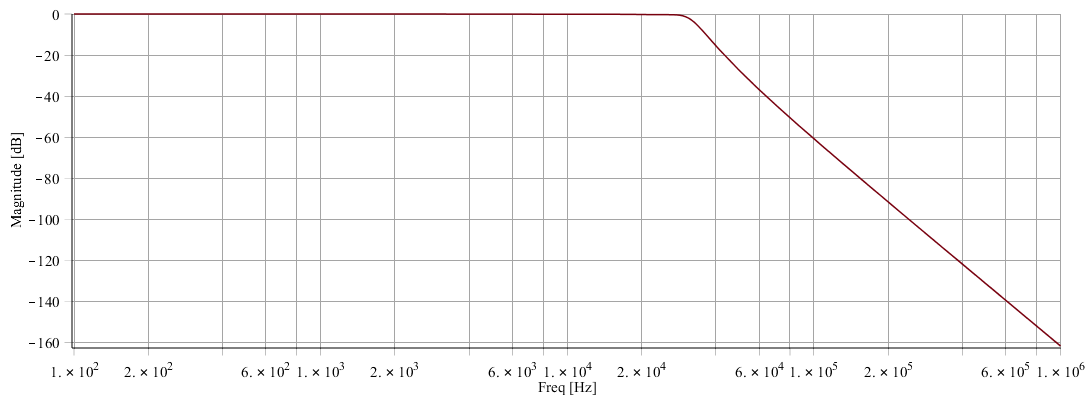
\includegraphics[width=\textwidth]{Imagenes-Ej1/legendre_hs.png}
	\end{subfigure}
	
	\begin{subfigure}{\textwidth}
	\centering
	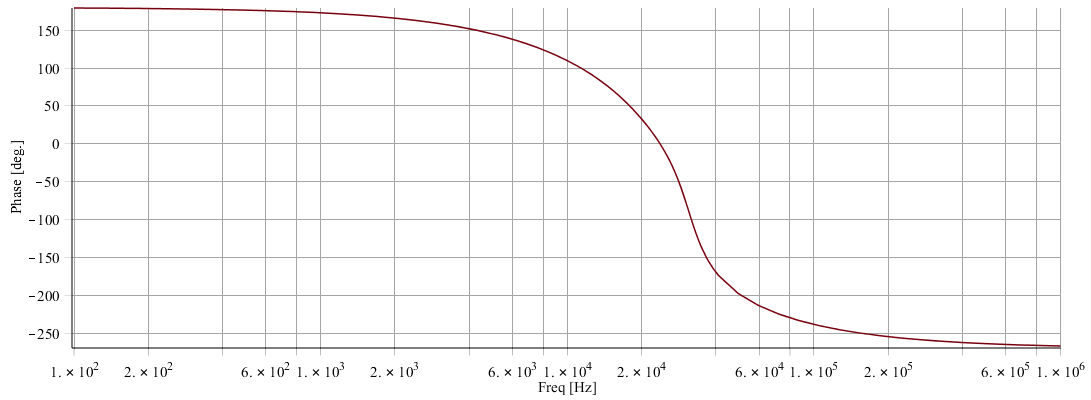
\includegraphics[width=\textwidth]{Imagenes-Ej1/legendre_hspha.png}
	\end{subfigure}
	\label{fig:bodebes}
	\caption{Diagrama de Bode del filtro aproximación Legendre.}
\end{figure}
y por último también con el software \textit{Maple}, el gráfico de polos y ceros:

\begin{figure}[H]
\centering
	\centering
	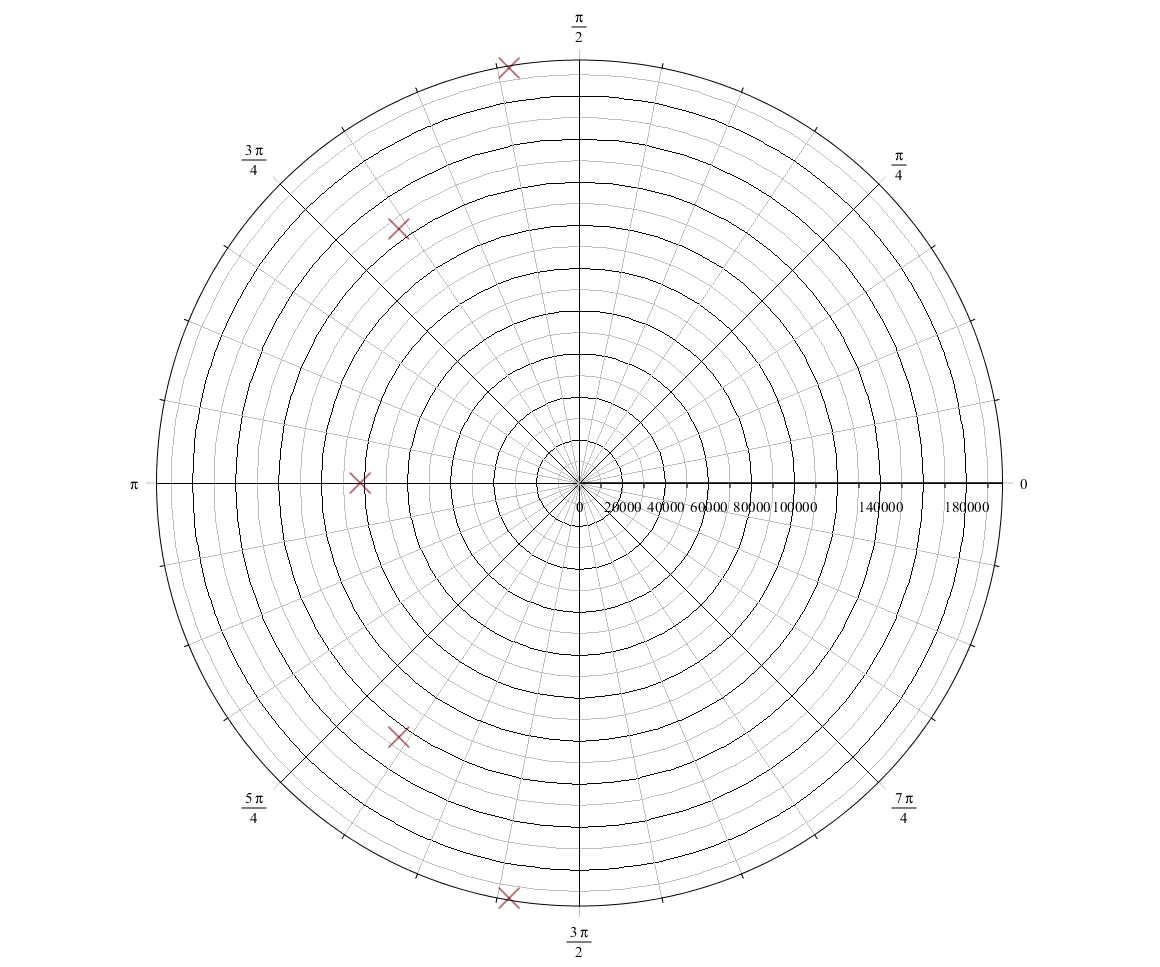
\includegraphics[width=0.8\textwidth]{Imagenes-Ej1/legendre_poles.png}
	\caption{Diagrama de polos y ceros del filtro aproximación Legendre}
	\label{leg_poles}
\end{figure}

\subsubsection{Elecciones de diseño}

Se utilizaron tres etapas, dos de segundo orden y una de primer orden. Para la etapa de primer orden, la de menor factor de calidad, se utilizó la configuración integradora compensada inversora. Para esta etapa se utilizaron valores de resistencias tales que la impedancia de entrada del filtro total sea mayor a los $50K\Omega$.

El ordenamiento de las etapas fue según factor de calidad creciente dado que las señales de entrada de este filtro serán de gran amplitud. Además, dado que la segunda etapa del filtro posee un gran sobrepico, se decidió atenuar en esta etapa y amplificar en la siguiente para reducir las chances de saturación en esta etapa y así disminuir la perdida de rango dinámico del filtro.

Los componentes utilizados para la realización del filtro junto a su implementación y error cometido son los siguientes:

\begin{table}[H]
\centering
\begin{tabular}{@{}cccccccc@{}}
\multicolumn{8}{c}{1ra Etapa - Integrador Compensado Inversor - Orden 1 - $f_0 = 16.23224KHz$ - $G=0dB$} \\ \midrule
- & Valor Teórico & Implementación & Valor Final & Error & Sens G  & Sens Wp \\ \midrule
$R_1 [\Omega]$ & $50K$ & $100K//100K$ & $50K$ & $0\%$ & -1 & 0 \\
$R_2 [\Omega]$ & $50K$ & $100K//100K$ & $50K$ & $0\%$ & 1 & -1 \\
$C_1 [F]$ & $196.1p$ & $220p+1.8n$ & $196.04p$ & $0.1\%$ & 0 & -1 \\
\bottomrule
\end{tabular}
\end{table}

\begin{table}[H]
\centering
\begin{tabular}{@{}cccccccc@{}}
\multicolumn{8}{c}{2da Etapa - Sallen-Key - Orden 2 - $f_0 = 31.2KHz$ - $G=-7dB$} \\ \midrule
- & Valor Teórico & Implementación & Valor Final & Error & Sens G & Sens Q & Sens Wp \\ \midrule
$R_1 [\Omega]$ & $21.43K$ & $22K//820K$ & $10K$ & $0.1\%$ & -0.6 & 0 & -0.2 \\
$R_2 [\Omega]$ & $8.53K$ & $330+8.2K$ & $8.53K$ & $0.1\%$ & 0 & 0 & -0.5 \\
$R_3 [\Omega]$ & $14.17K$ & $2.2K+12K$ & $14.2K$ & $0.2\%$ & 0.6 & 0 & -0.3 \\
$C_1 [F]$ & $3.58n$ & $4.7n+15n$ & $3.58n$ & $0.1\%$ & 0 & 0.5 & -0.5 \\
$C_2 [F]$ & $100p$ &  & $100p$ & $0\%$ & 0 & -0.5 & -0.5 \\ \bottomrule
\end{tabular}
\end{table}
 
\begin{table}[H]
\centering
\begin{tabular}{@{}cccccccc@{}}
\multicolumn{8}{c}{3ra Etapa - Sallen-Key - Orden 2 - $f_0 = 23KHz$ - $G=7dB$} \\ \midrule
- & Valor Teórico & Implementación & Valor Final & Error & Sens G & Sens Q & Sens Wp \\ \midrule
$R_1 [\Omega]$ & $57.31K$ & $1.2K+56K$ & $57.2K$ & $0.2\%$ & 0 & 0.54 & -0.2 \\
$R_2 [\Omega]$ & $57.31K$ & 1.2K+56K & $57.2K$ & $0.2\%$ & 0 & -0.54 & -0.5 \\
$R_3 [\Omega]$ & $1K$ &  & $1K$ & $0\%$ & -0.6 & -1.08 & 0 \\
$R_4 [\Omega]$ & $1.72K$ & $12+1.5K$ & $1.51K$ & $0.1\%$ & 0.6 & 1.08 & 0 \\
$C_1 [F]$ & $100p$ &  & $100p$ & $0\%$ & 0 & 1.58 & -0.5 \\
$C_2 [F]$ & $145.32p$ & $150p+4.7n$ & $145.36p$ & $0.1\%$ & 0 & -1.58 & -0.5 \\ \bottomrule
\end{tabular}
\end{table}

\subsubsection{Acoplamiento de Impedancias.}
Dado que la primera etapa posee a la entrada una resistencia serie de $50K\Omega$ se asegura que el filtro cumpla con la restricción de $|Z_{in}| \geq 50K\Omega$. Luego, como la celda con la que se trabaja posee una impedancia de salida extremadamente baja, habrá un buen acoplamiento de impedancias.

\subsubsection{Simulaciones}

Se simuló utilizando el operacional $TL-081$ y el software \textit{LTSpiceXVII} la respuesta en frecuencia, impedancia de entrada, impedancia de salida y finalmente el montecarlo para el filtro diseñado.

\begin{figure}[H]
\centering
	\centering
	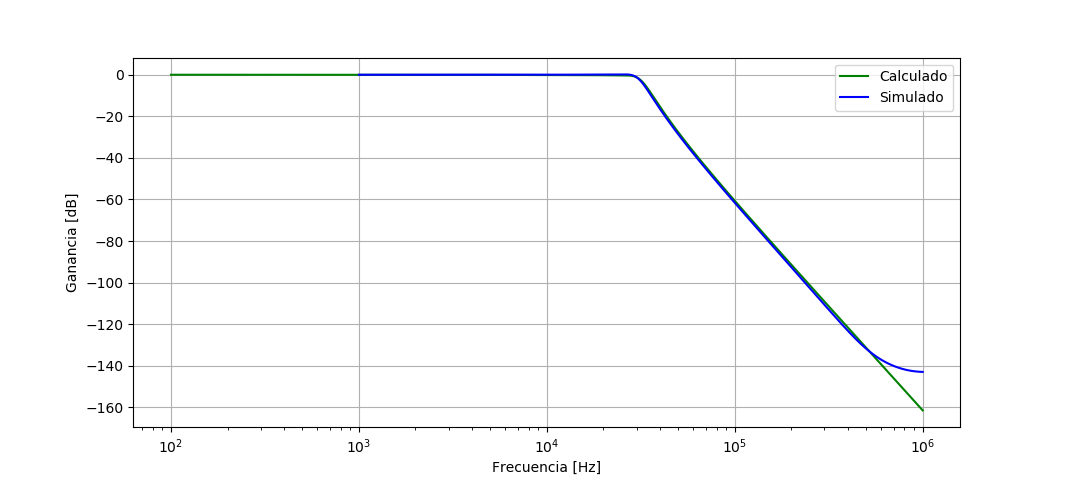
\includegraphics[width=\textwidth]{Imagenes-Ej1/legendre_hs_sim.png}
	\caption{Simulación de la respuesta en frecuencia en amplitud del filtro aproximación Legendre.}
	\label{leg_gain_sim}
\end{figure}

\begin{figure}[H]
\centering
	\centering
	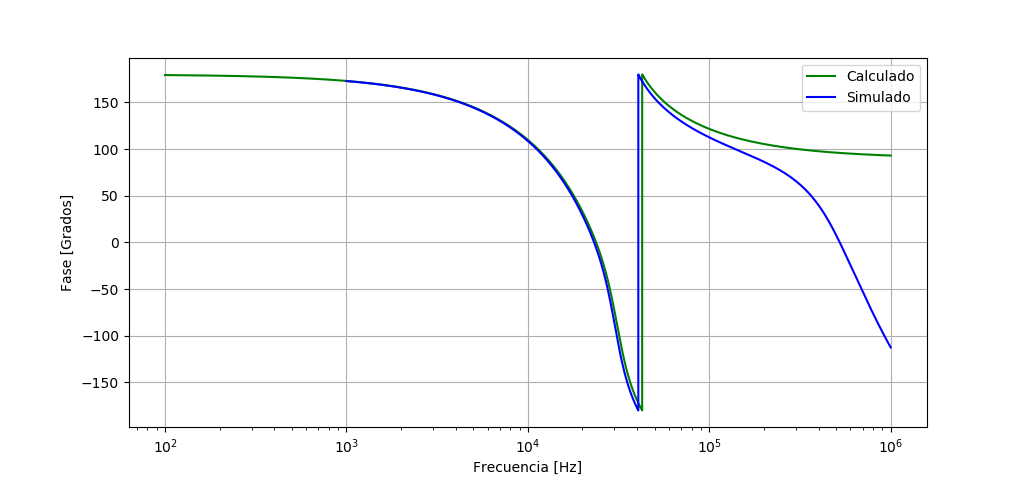
\includegraphics[width=\textwidth]{Imagenes-Ej1/legendre_hspha_sim.png}
	\caption{Simulación de la respuesta en frecuencia en fase del filtro aproximación Legendre.}
	\label{leg_phase_sim}
\end{figure}

\begin{figure}[H]
\centering
	\centering
	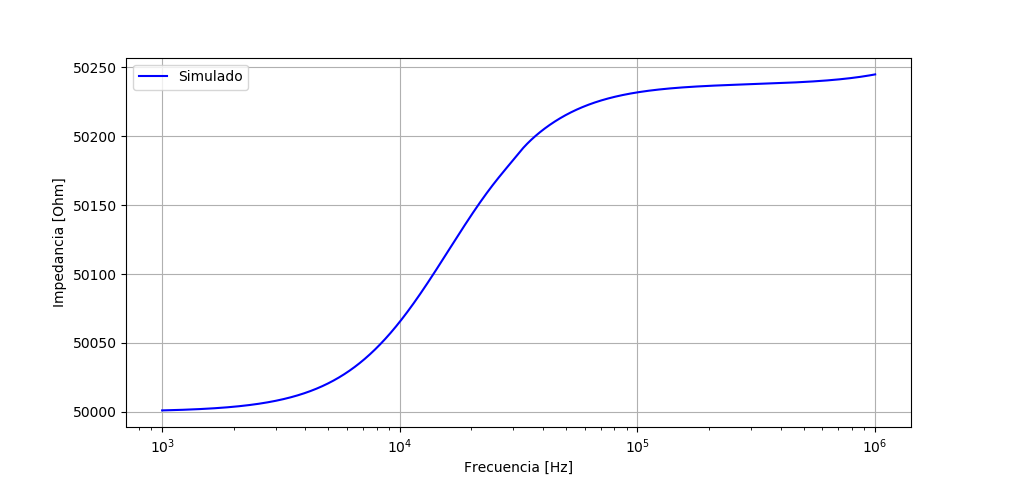
\includegraphics[width=\textwidth]{Imagenes-Ej1/legendre_zin_sim.png}
	\caption{Simulación de la impedancia de entrada del filtro aproximación Legendre.}
	\label{leg_zin_sim}
\end{figure}

\begin{figure}[H]
\centering
	\centering
	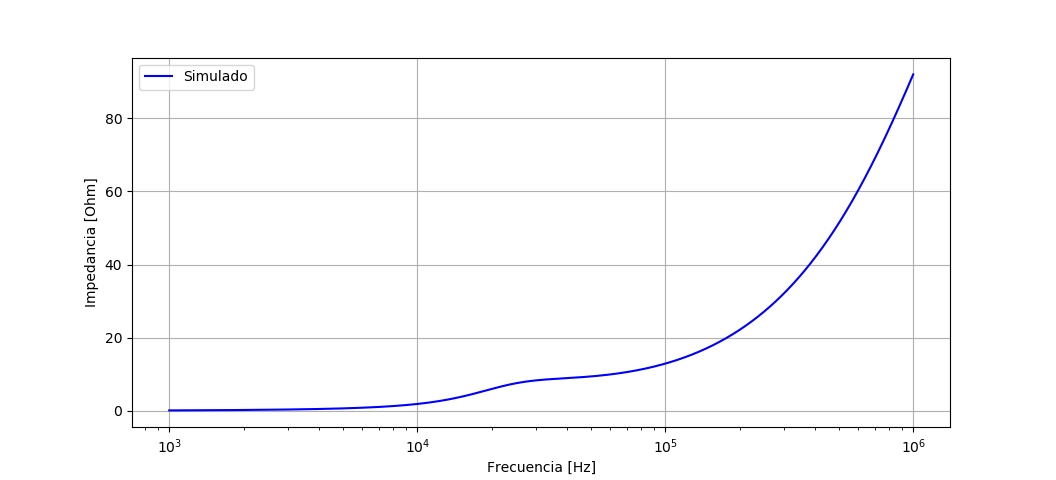
\includegraphics[width=\textwidth]{Imagenes-Ej1/legendre_zout_sim.png}
	\caption{Simulación de la impedancia de salida del filtro aproximación Legendre.}
	\label{leg_zout_sim}
\end{figure}

\begin{figure}[H]
\centering
	\centering
	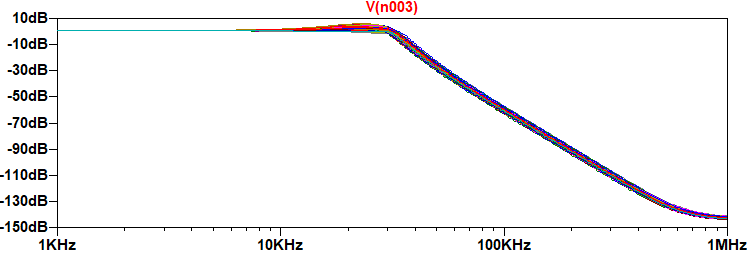
\includegraphics[width=\textwidth]{Imagenes-Ej1/legendre_mont.png}
	\caption{Simulación de Montecarlo del filtro aproximación Legendre.}
	\label{leg_mont_sim}
\end{figure}

Se puede observar en el montecarlo del filtro realizado con la aproximación Legendre con tolerancias del \%1  para resistencias y \%10 para los capacitores que solamente cuatro en cien curvas no cumplen con la plantilla utilizada por lo que se optó a no utilizar presets en la celda midiendo por separado los valores de las resistencias y capacitores más sensibles.

\subsubsection{Rango Dinámico}

Para el rango dinámico se utilizó la ganancia máxima de $2.238721$ y una ganancia mínima de $0.446684$. Luego, la tensión de entrada máxima será
\begin{equation}
V_{i_{max}}= \frac{V_{o_{max}}}{2.238721}
\end{equation}
y la tensión mínima de entrada será
\begin{equation}
V_{i_{min}}= \frac{V_{o_{min}}}{0.446684}
\end{equation}
y considerando que nuestra tensión máxima es de $13.5V$ fijada por la saturación del opamp y nuestro piso de ruido se encuentra en los $10mV$, el rango dinámico será
\begin{equation}
DR=20log(\frac{V_{i_{max}}}{V_{i_{min}}}) = 48.6dB
\end{equation}


\subsubsection{Mediciones}



\subsection{Aproximación de Bessel.}

Para cumplir con la plantilla propuesta con seguridad, se diseñó el filtro con una plantilla más restrictiva que la original, presentada a continuación.
\begin{figure}[H]
		\begin{table}[H]
			\centering
			\begin{tabular}{@{}cc@{}}
			\toprule
			\multicolumn{2}{c}{Large Signal LP Sallen-Key Bessel} \\ \midrule
			$f_p$ & $1650Hz$ \\
			$f_a$ & $7800Hz$ \\
			$A_p$ & $2dB$ \\
			$A_a$ & $43dB$ \\
			$\Upsilon$ & $\leq 5\%$ \\
			$\left| Z_{in}\right|$ & $\geq 50K\Omega$ \\ \bottomrule
			\end{tabular}
		\end{table}
		\caption{Aproximación de Bessel más estricta utilizada.}
		\label{aprox_leg_est}
\end{figure}

Por lo que la transferencia total del filtro de esta plantilla es:

\begin{equation}
\hspace{-1cm}
H(s) = \frac{1}{s^6 \cdot 9.0334\cdot10^{-27}+s^5\cdot 8.8909\cdot10^{-22}+s^4\cdot 4.1690\cdot10^{-17}+s^3\cdot 1.1731\cdot10^{-12}+s^2\cdot 2.0632\cdot10^{-8}+s\cdot 2.1292\cdot10^{-4}+1}
\label{hsbesteo}
\end{equation}

Luego, se graficó el diagrama de Bode con el software \textit{Maple}, resultando:
\begin{figure}[H]
	\begin{subfigure}{\textwidth}
	\centering
	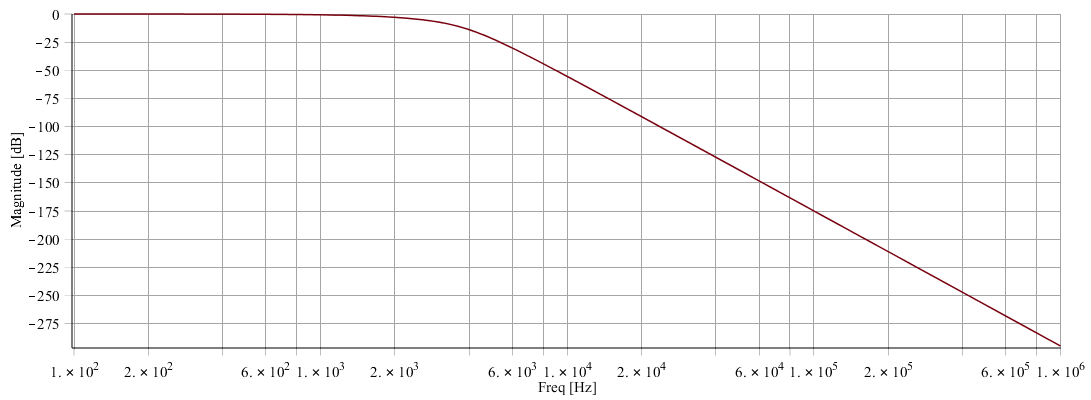
\includegraphics[width=\textwidth]{Imagenes-Ej1/bessel_hs.png}
	\end{subfigure}
	
	\begin{subfigure}{\textwidth}
	\centering
	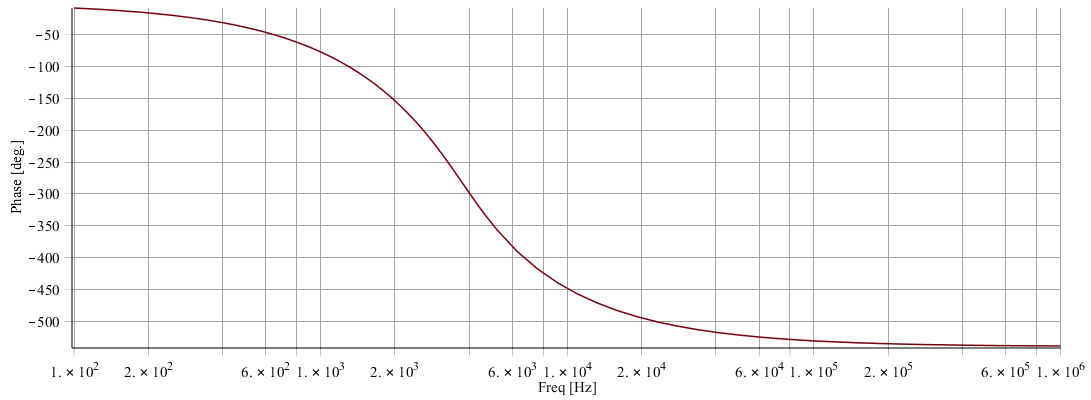
\includegraphics[width=\textwidth]{Imagenes-Ej1/bessel_hspha.png}
	\end{subfigure}
	\label{fig:bodebes}
	\caption{Diagrama de Bode del filtro aproximación Bessel.}
\end{figure}
También se realizó el gráfico de polos y ceros con el software \textit{Maple}:

\begin{figure}[H]
\centering
	\centering
	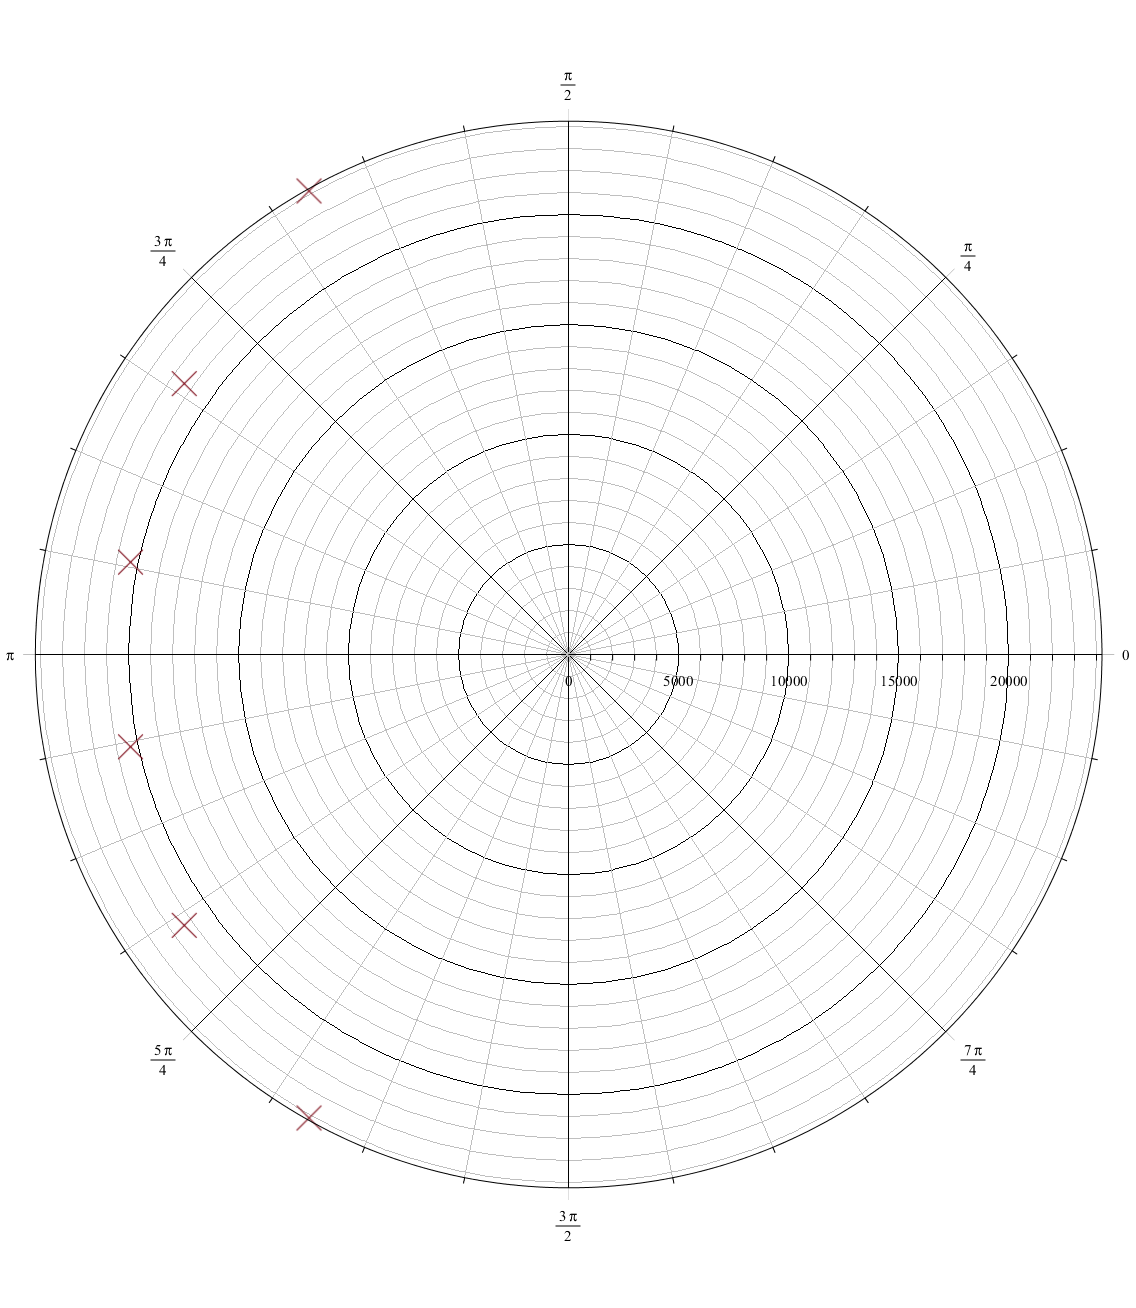
\includegraphics[width=0.7\textwidth]{Imagenes-Ej1/bessel_poles.png}
	\caption{Diagrama de polos y ceros del filtro aproximación Bessel}
	\label{leg_poles}
\end{figure}

y finalmente el gráfico del group delay.

\begin{figure}[H]
\centering
	\centering
	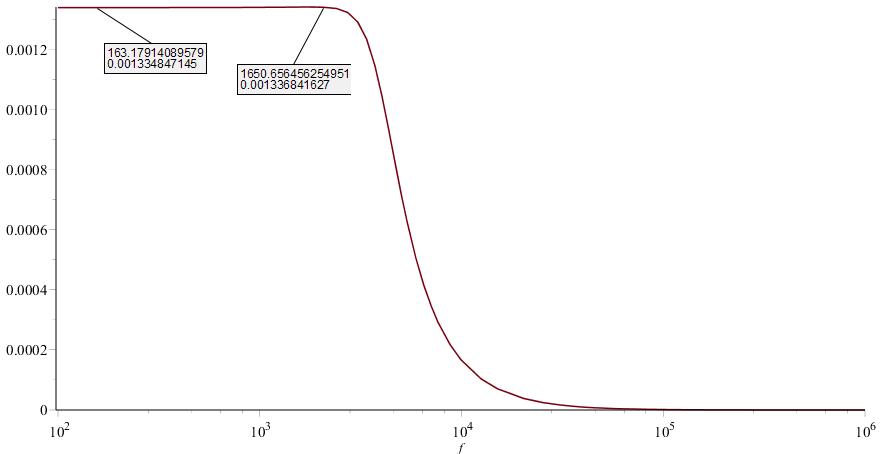
\includegraphics[width=\textwidth]{Imagenes-Ej1/groupdelay_calc.png}
	\caption{Group delay del filtro aproximación Bessel.}
	\label{bes_group_calc}
\end{figure}

El desvío del group-delay se encuentra por debajo del $5\%$ y es de $\approx 0.149\%$.

\subsubsection{Elecciones de diseño}

Para la implementación de esta aproximación se utilizaron nuevamente tres etapas, las tres de segundo orden. Dado que las señales de entrada esperadas en este filtro serán pequeñas, se decidió utilizar un ordenamiento de las etapas con un factor de calidad decreciente para favorecer la reducción de ruido. Además, se decidió amplificar en la primera etapa y atenuar en la última.

Los componentes utilizados para la realización del filtro junto a su implementación y error cometido son los siguientes:

\begin{table}[H]
\centering
\begin{tabular}{@{}cccccccc@{}}
\multicolumn{8}{c}{1ra Etapa - Sallen-Key - Orden 2 - $f_0 = 3.2KHz$ - $G=7dB$} \\ \midrule
- & Valor Teórico & Implementación & Valor Final & Error & Sens G & Sens Q & Sens Wp \\ \midrule
$R_1 [\Omega]$ & $50K$ & $100K//100K$ & $50K$ & $0\%$ & 0 & 0.15 & -0.5 \\
$R_2 [\Omega]$ & $50K$ & $100K//100K$ & $50K$ & $0\%$ & 0 & -0.15 & -0.5 \\
$R_3 [\Omega]$ & $603.9$ & $680//5K6$ & $606.37$ & $0.4\%$ & -0.44 & -0.31 & 0 \\
$R_4 [\Omega]$ & $470$ &  & $470$ &  & 0.44 & 0.31 & 0 \\
$C_1 [F]$ & $766.98p$ & $1000p+3.3n$ & $767.44p$ & $0.1\%$ & 0 & 0.81 & -0.5 \\
$C_2 [F]$ & $1.26n$ & $68p//1.2n$ & $1.27n$ & $0.4\%$ & 0 & -0.81 & -0.5 \\ \bottomrule
\end{tabular}
\end{table}

\begin{table}[H]
\centering
\begin{tabular}{@{}cccccccc@{}}
\multicolumn{8}{c}{2da Etapa - Sallen-Key - Orden 2 - $f_0 = 3.4KHz$ - $G=0dB$} \\ \midrule
- & Valor Teórico & Implementación & Valor Final & Error & Sens G & Sens Q & Sens Wp \\ \midrule
$R_1 [\Omega]$ & $4.7K$ & $Preset$ & $10K$ & $0\%$ & 0 & 0 & -0.5 \\
$R_2 [\Omega]$ & $4.7K$ &  & $4.7K$ & $0\%$ & 0 & 0 & -0.5 \\
$C_1 [F]$ & $12.15n$ & $150p//12n$ & $12.15n$ & $0\%$ & 0 & 0.5 & -0.5 \\
$C_2 [F]$ & $8.13n$ & $8.2n+1u$ & $8.13n$ & $0\%$ & 0 & -0.5 & -0.5 \\ \bottomrule
\end{tabular}
\end{table}
 
\begin{table}[H]
\centering
\begin{tabular}{@{}cccccccc@{}}
\multicolumn{8}{c}{3ra Etapa - Sallen-Key - Orden 2 - $f_0 = 3.8KHz$ - $G=-7dB$} \\ \midrule
- & Valor Teórico & Implementación & Valor Final & Error & Sens G & Sens Q & Sens Wp \\ \midrule
$R_1 [\Omega]$ & $2.13K$ & $3.9K//4.7K$ & $2.13K$ & $0\%$ & -0.44 & 0 & -0.28 \\
$R_2 [\Omega]$ & $1.2K$ &  & $1.2K$ & $0\%$ & 0 & 0 & -0.5 \\
$R_3 [\Omega]$ & $2.74K$ & $39+2.7K$ & $2.74K$ & $0\%$ & 0.44 & 0 & -0.22 \\
$C_1 [F]$ & $70.67n$ & $2.7n//68n$ & $70.7n$ & $0.1\%$ & 0 & 0.5 & -0.5 \\
$C_2 [F]$ & $16.87n$ & $1n//6.8n$ & $16.80n$ & $0.2\%$ & 0 & -0.5 & -0.5 \\ \bottomrule
\end{tabular}
\end{table}

\subsubsection{Acoplamiento de Impedancias.}
Dado que la primera etapa posee a la entrada una resistencia serie de $50K\Omega$ se asegura que el filtro cumpla con la restricción de $|Z_{in}| \geq 50K\Omega$. Luego, como la celda con la que se trabaja posee una impedancia de salida extremadamente baja, habrá un buen acoplamiento de impedancias.

\subsubsection{Simulaciones}

Se simuló utilizando el operacional $TL-081$ y el software \textit{LTSpiceXVII} la respuesta en frecuencia, impedancia de entrada, impedancia de salida y finalmente el montecarlo para el filtro diseñado.

\begin{figure}[H]
\centering
	\centering
	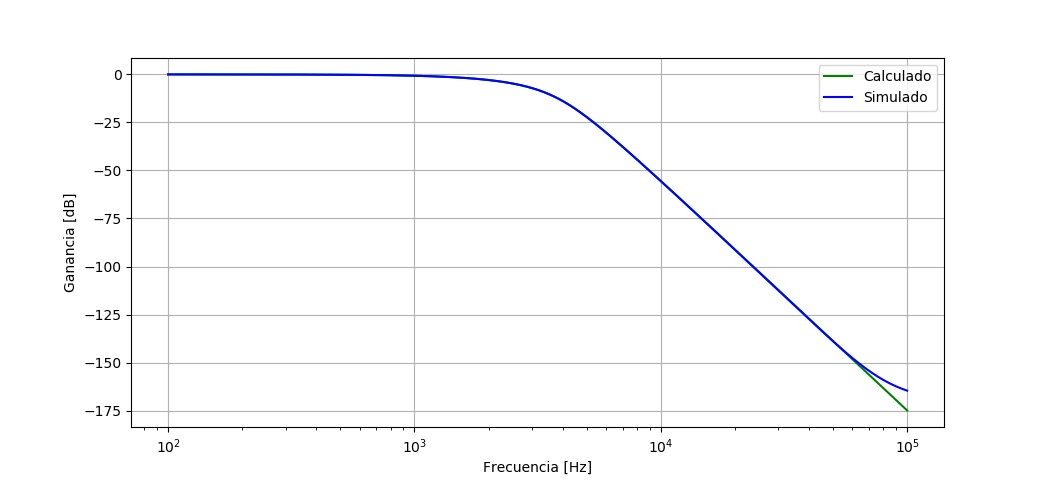
\includegraphics[width=\textwidth]{Imagenes-Ej1/bessel_hs_sim.png}
	\caption{Simulación de la respuesta en frecuencia en amplitud del filtro aproximación Bessel.}
	\label{bes_gain_sim}
\end{figure}

\begin{figure}[H]
\centering
	\centering
	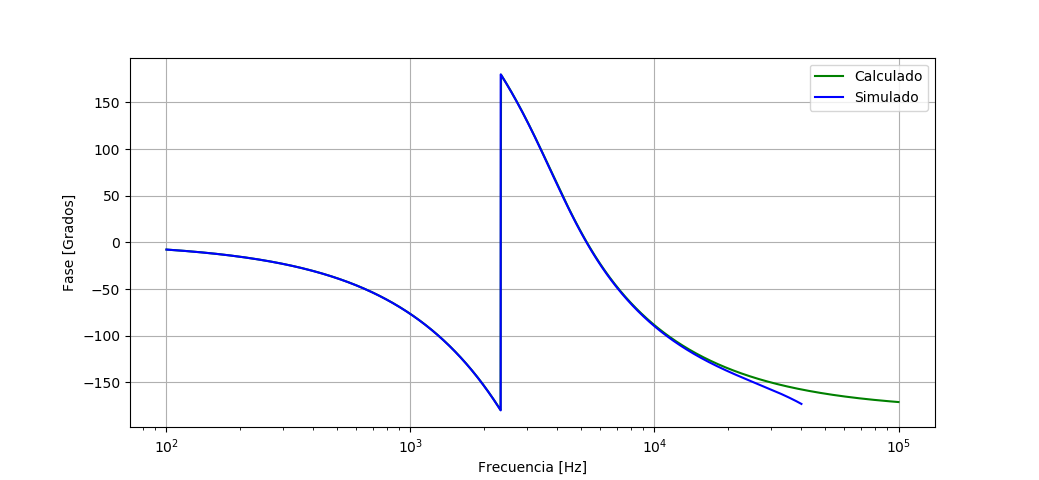
\includegraphics[width=\textwidth]{Imagenes-Ej1/bessel_hspha_sim.png}
	\caption{Simulación de la respuesta en frecuencia en fase del filtro aproximación Bessel.}
	\label{bes_phase_sim}
\end{figure}

\begin{figure}[H]
\centering
	\centering
	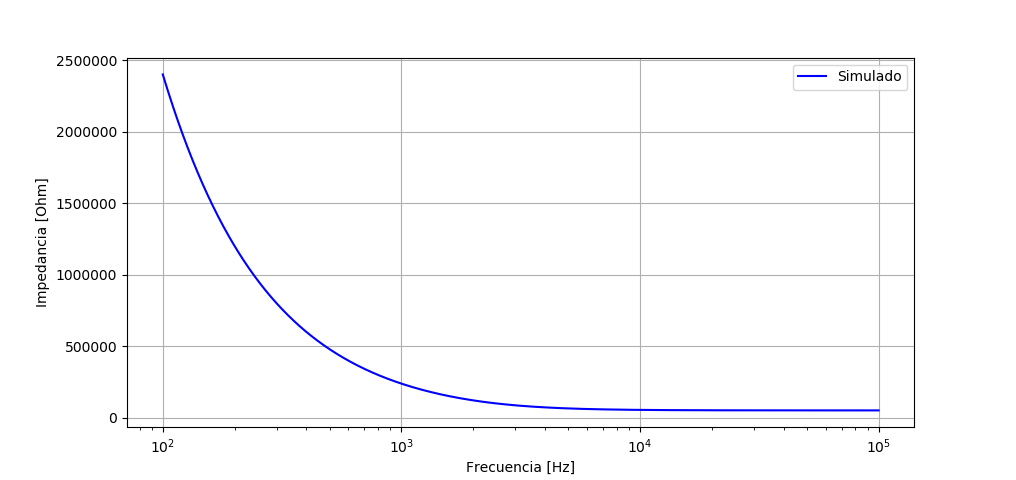
\includegraphics[width=\textwidth]{Imagenes-Ej1/bessel_zin_sim.png}
	\caption{Simulación de la impedancia de entrada del filtro aproximación Bessel.}
	\label{bes_zin_sim}
\end{figure}

\begin{figure}[H]
\centering
	\centering
	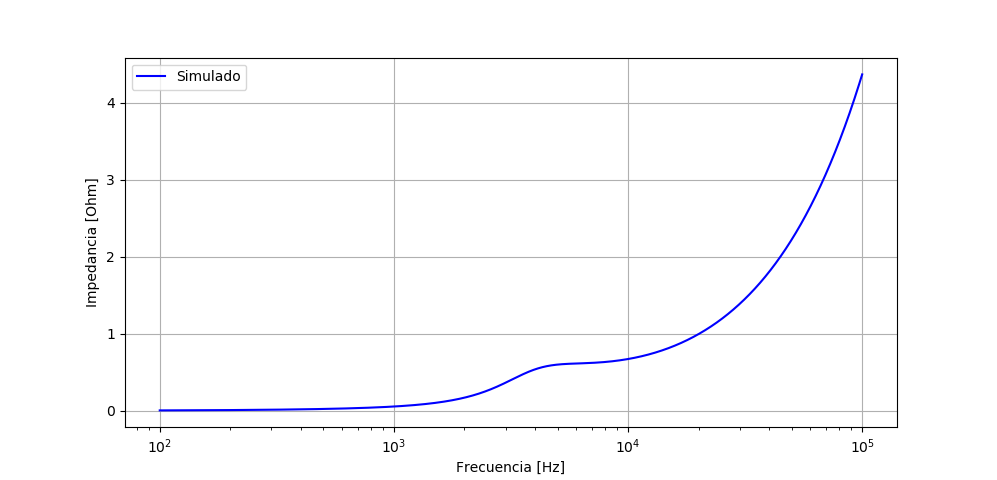
\includegraphics[width=\textwidth]{Imagenes-Ej1/bessel_zout_sim.png}
	\caption{Simulación de la impedancia de salida del filtro aproximación Bessel.}
	\label{bes_zout_sim}
\end{figure}

\begin{figure}[H]
\centering
	\centering
	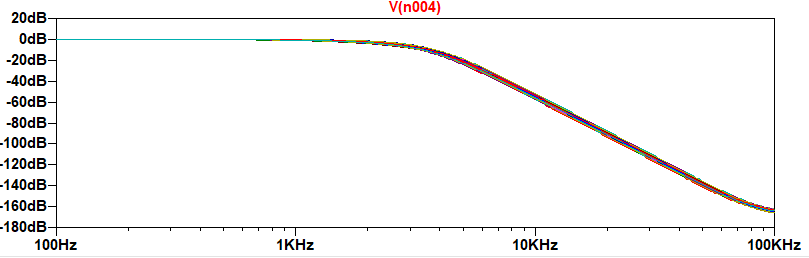
\includegraphics[width=\textwidth]{Imagenes-Ej1/bessel_mont.png}
	\caption{Simulación de montecarlo del filtro aproximación Bessel.}
	\label{bes_mont_sim}
\end{figure}

Se puede observar en el montecarlo del filtro realizado con la aproximación Bessel con tolerancias del \%1  para resistencias y \%10 para los capacitores que todas las curvas cumplen con la plantilla utilizada por lo que se optó a no utilizar presets en la celda midiendo por separado los valores de las resistencias y capacitores más sensibles.


\subsubsection{Rango Dinámico}

Para el rango dinámico se utilizó la ganancia máxima de $2.238721$ y una ganancia mínima de $0.446684$. Luego, la tensión de entrada máxima será
\begin{equation}
V_{i_{max}}= \frac{V_{o_{max}}}{2.238721}
\end{equation}
y la tensión mínima de entrada será
\begin{equation}
V_{i_{min}}= \frac{V_{o_{min}}}{0.446684}
\end{equation}
y considerando que nuestra tensión máxima es de $13.5V$ fijada por la saturación del opamp y nuestro piso de ruido se encuentra en los $10mV$, el rango dinámico será
\begin{equation}
DR=20log(\frac{V_{i_{max}}}{V_{i_{min}}}) = 48.6dB
\end{equation}


\subsubsection{Mediciones}


\subsection{Conclusiones}



\subsection{Anexo de Sensibilidades}
\begin{equation}
S^{G}_{C_2}={{\it C2}\,{\pi }^{2}\\
\mbox{}{f}^{2} \left( {\it R2}+{\it R1} \right)  \left( {\it C2}\, \left( {\it R2}+{\it R1} \right) -{\frac {{\it C1}\,{\it R1}\,{\it R4}}{{\it R3}}}\\
\mbox{} \right)  \left(  \left( -4\,{\pi }^{2}{f}^{2}{\it R2R1C2C1}+1 \right) ^{2}+4\,{\pi }^{2}{f}^{2} \left( {\it C2}\, \left( {\it R2}+{\it R1} \right) -{\frac {{\it C1}\,{\it R1}\,{\it R4}}{{\it R3}}} \right) ^{2} \right) ^{-1}}
\end{equation}
\end{document}